\documentclass{report}
\usepackage[margin=1in, paperwidth=8.5in, paperheight=11in]{geometry}
%Math packages%
\usepackage{amsmath}
\usepackage{amsthm}
%Spacing%
\usepackage{setspace}
%Package to adjust indentation%
\usepackage{changepage}
\onehalfspacing
%Lecture number%
\newcommand{\lectureNum}{16}
%Variables - Date and Course%
\newcommand{\curDate}{March 7, 2017}
\newcommand{\course}{CS 240}
%Defining the example tag%
%\theoremstyle{definition}%
\newtheorem{ex}{Example}[section]
%Setting counter given the lecture number%
\setcounter{chapter}{\lectureNum{}}
%Package to insert code%
\usepackage{listings}
\usepackage{courier}
\usepackage{xcolor}
\lstset { 
    tabsize=2,
    breaklines=true,
    language=C++,
    backgroundcolor=\color{blue!8}, % set backgroundcolor
    basicstyle=\footnotesize\ttfamily,% basic font setting
}
%Package to draw trees%
\usepackage{tikz}


\begin{document}
%Note title%
\begin{center}
\begin{Large}
\textsc{\course{} | Lecture \lectureNum{}}
\end{Large}
\end{center} 
\noindent \textit{Bartosz Antczak} \hfill
\textit{Instructor: Troy Vasiga} \hfill
\textit{\curDate{}}
\rule{\textwidth}{0.4pt}

% Actual Notes%
\section{More on 2-D Range Search}
\subsection{Kd-trees}
\subsubsection{Search complexity}
We define $Q(n)$ to be the maximum number of regions in a kd-tree with $n$ points that intersect a vertical (horizontal) line. $Q(n)$ satisfies
$$Q(n) = 2Q(n/4) + O(1)$$
It solves that $Q(n) = O(\sqrt{n})$.
\subsection{Range Trees}
We have $n$ points $P = \{(x_0, y_0), (x_1, y_1), \cdots, (x_{n-1}, y_{n-1})\}$. A range tree is a \textit{tree of trees}. This tree is determined by the $x-$coordinates. We build it using the following steps:
\begin{itemize}
\item Build a balanced binary search tree $\tau$ determined by the $x-$coordinates
\item For every node $v \in \tau$, build a balanced binary search tree $\tau_{assoc}(v)$ (associated structure of $\tau$) determined by the $y-$coordinates of the nodes in the subtree of $\tau$ with root node $v$
\end{itemize}
\begin{ex}
A sample range tree. This tree is ordered by the x-coordinates (i.e., all x values less than the root's x-value are to the left, and the greater values to the right)
\end{ex}
\begin{center}
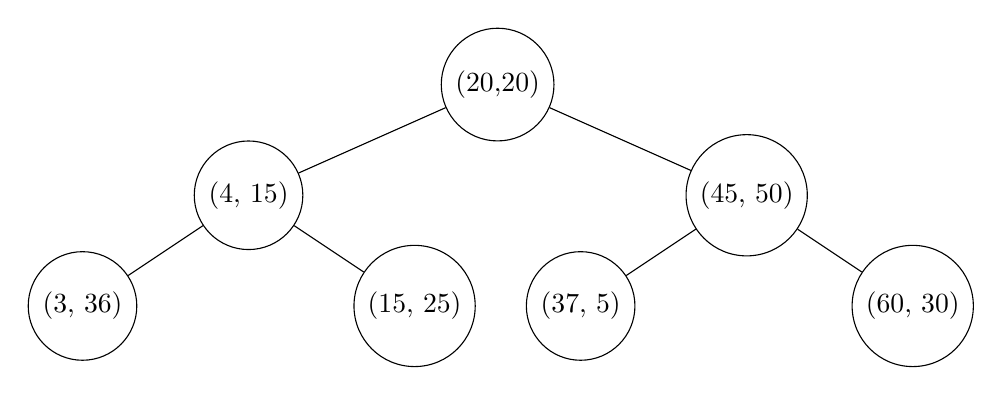
\begin{tikzpicture}[
  level distance=40 pt,
  every node/.style={circle,draw},
  level 1/.style={sibling distance=180 pt},
  level 2/.style={sibling distance=120 pt},
  level 3/.style={sibling distance=120 pt}
]
  \node {(20,20)}
  	child {node {(4, 15)}
  		child {node {(3, 36)}}
  		child {node {(15, 25)}}}
  	child {node {(45, 50)}
  		child {node {(37, 5)}}
  		child {node {(60, 30)}}};
\end{tikzpicture}
\end{center}
Now if we consider the node (4, 15), we will draw its associated tree ($\tau_{(4, 15)}$):
\begin{center}
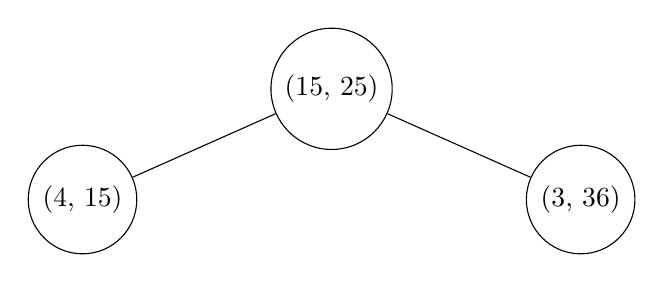
\begin{tikzpicture}[
  level distance=40 pt,
  every node/.style={circle,draw},
  level 1/.style={sibling distance=180 pt},
  level 2/.style={sibling distance=120 pt},
  level 3/.style={sibling distance=120 pt}
]
  \node {(15, 25)}
  	child {node {(4, 15)}}
  	child {node {(3, 36)}};
\end{tikzpicture}
\end{center}
In short, every node in a range tree has two sets of children that compose of two different trees ($\tau$ and $\tau_{assoc}$). One tree orders all of its children plus the root based on the order on the $x$ and $y$ coordinates respectively.
\subsubsection{Range Tree Operations}
\begin{itemize}
\item \texttt{Search}: trivially as in a binary search tree ($O(\log n$)
\item \texttt{Insert}: insert a point in $\tau$ by $x-$coordinate. From the inserted leaf, walk back up to the root and insert the point in all associated trees $\tau_{assoc}(v)$ of nodes $v$ on path to the root (there are $\log n$ trees and each insertion takes $O(\log n)$. So our running time is $O(\log^2 n)$)
\item \texttt{Delete:} analogous to insertion
\end{itemize}
Note: rebalancing a range tree will be problematic! We must use another method, which we will not cover in this course.\\The main operation which will concern us will be range search.
\subsection{Range Search on a Range Tree}
It is a two stage process. To perform a range search query $R = [x_1, x_2] \times [y_1, y_2]$:
\begin{itemize}
\item Perform a range search (on the $x-$coordinates) for the interval $[x_1, x_2]$ in $\tau$
\item For every outside node, do nothing ($O(1)$)
\item For every ``top" inside node $v$, perform a range search (on the $y-$coordinates) for the interval $[y_1, y_2]$ in $\tau_{assoc}(v)$. During the range search of $\tau_{assoc}(v)$, do not check any $x-$coordinates (they are all within range) ($\log n \times \log n = O(\log^2 n)$)
\item For every boundary node, test to see if the corresponding point is within the region $R$ ($O(\log n)$)
\end{itemize}
The running time of search if $O(k + \log^2 n)$. We need $O(n \log n)$ space. Why do we need that much space? Intuitively, you'd think we would need $O(n^2)$ space, but think about it: there are $n$ nodes, and each node is in at most $\log n$ trees, ergo $O(n \log n)$. $\log^2 n < \sqrt{n}$.
\subsection{Higher Dimensions}
For every node, there are a total of $d$ trees (where $d$ is the dimension).
\begin{figure}[ht]
\begin{center}
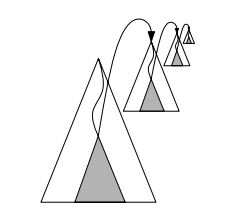
\includegraphics[scale=0.7]{dimen.jpg}
\end{center}
\caption{A 4-dimensional tree}
\end{figure}
\section{Tries and String Matching}
I sense this will merge topics with CS 241 (and the first few weeks of CS 246 too).
\subsection{Pattern Matching}
Involves searching for a string in a large body of text. Say our text is in $T[0, \cdots, n-1]$ (the \textit{haystack}), and our pattern is $P[0, \cdots, m-1]$ (the \textit{needle}). These strings are over the alphabet $\Sigma$. We want to return the first $i$ such that
$$P[j] = T[i+j] \quad (0 \leq j \leq m-1)$$
This is the first occurrence of $P$ in $T$. If $P$ does not occur in $T$, then we return \texttt{FAIL}.\\Some applications involving pattern matching include:
\begin{itemize}
\item Information Retrieval (text editors, search engines)
\item Bioinformatics (your DNA is nothing more than C, G, T, A)
\item Data Mining
\end{itemize}
\begin{ex}
Pattern matching on a particular string
\end{ex}
\begin{itemize}
\item $T = $ ``Where is he?"
\item $P_1 = $ ``he"
\item $P_2 = $ ``who"
\end{itemize}
The search for $P_1$ returns 1 (index 1 in $T$), and the search for $P_2$ returns \textbf{FAIL}.
\subsubsection{Some Definitions}
\begin{itemize}
\item \textbf{Prefix}: a substring $T[0 ... i]$ of $T$
\item \textbf{Suffix}: a substring $T[i ... n-1]$ of $T$
\end{itemize}
\subsection{General Idea of Pattern Matching Algorithms}
Pattern matching algorithms consist of guesses and checks:
\begin{itemize}
\item A \textbf{guess} is a position $i$ such that $P$ might start at $T[i]$
\item A \textbf{check} of a guess is a single position $j$ with $0 \leq j < m$ where we compare $T[i+j]$ to $P[j]$. We must perform $m$ checks of a single correct guess, but we may make (many) fewer checks of an incorrect guess
\end{itemize}
So how do we implement these algorithms?
\subsection{Approach 1: brute force}
We scan the entire string and check every index. We start at the 0th index, and check every single one until we match:
\begin{figure}[ht]
\begin{center}
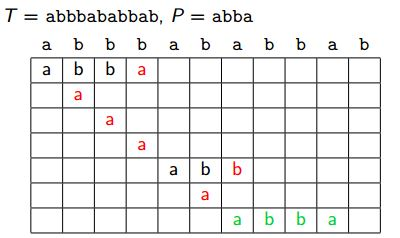
\includegraphics[scale=0.8]{brute.jpg}
\end{center}
\end{figure}
Obviously, we can better than brute force. We will focus on four, more sophisticated algorithms. We'll dive into them starting in the next lecture.

%END%
\end{document}